\documentclass[times, utf8, zavrsni]{fer}
\usepackage{booktabs}
\usepackage[section]{placeins}
\usepackage{float		}


\begin{document}

% TODO: Navedite broj rada.
\thesisnumber{000}

% TODO: Navedite naslov rada.
\title{Programska podrška za svršenike}

% TODO: Navedite vaše ime i prezime.
\author{Tomislav Kravaršćan}

\maketitle

% Ispis stranice s napomenom o umetanju izvornika rada. Uklonite naredbu \izvornik ako želite izbaciti tu stranicu.
\izvornik

% Dodavanje zahvale ili prazne stranice. Ako ne želite dodati zahvalu, naredbu ostavite radi prazne stranice.
\zahvala{}

\tableofcontents

\chapter{Uvod}
Svršenici (lat. \textit{alumni}) je popularan naziv za bivše pripadnike neke ustanove, najčešće sveučilišta. Alumni su uobičajena udruženja u svijetu pa u nekim sveučilištima imaju i stoljetnu tradiciju. Njihovo ponovno okupljanje i sudjelovanje u radu sveučilišta je vrlo bitno za održavanje priče o prošlosti, a i za planiranje budućnosti sveučilišta. No, kako studenti sveučilišta vrlo brzo nakon diplomiranja utonu u nove životne prilike kao što su posao i obitelj, fakultetima je vrlo teško održavati vezu sa svojim bivšim studentima i ponovno ih okupljati. A i sami se svršenici teško održe na okupu. Za to je rješenje programska podrška u obliku društvene web aplikacije, gdje će se moći organizirati događaji, sastanci i objavljivati razne objave vezane za svršenike.

\chapter{Analiza postojeće programske podrške}
Analizom postojeće programske potpore nastojimo bolje razumijeti problem koji rješavamo, njegovu domenu primjene i razrješiti moguće krive početne pretpostavke o programskoj podršci koju izrađujemo. Također, jasnije vidimo funkcionalnosti koje bi trebali implementirati i dobivamo ideje o nekim detaljima o kojima uopće nismo razmišljali. Osim toga, svrha analize je i otrkivanje mogućih nedostataka koje trpi posojeća programska podrška, te učenje na tuđim pogreškama. Moramo biti posebno svjesni kojim su resursima raspolagali razvojni inženjeri analiziranih rješenja kako bismo što ranije odredili doseg našeg rješenja sukladno našim resursima vremena i znanja.
U ovom konkretnom slučaju, analizirati ćemo programska rješenja za upravljanje svršenicima. Takvih rješenja ima neiscrpno puno pa ćemo navesti samo neka od njih. Gotovo sva postojeća rješenja nude neke osnovne funkcionalnosti kao što su organizacija i pregled događaja, pregled novosti, informacije o sustavu, ponuda poslova, stvaranje i upravljanje korisničkim računom.

\section{Graduway}
Graduway[1] je web platforma istoimene tvrtke koja za različite fakultete po narudžbi stvara aplikaciju prilagođenu određenoj ustanovi za koju se izrađuje. Uz gore navedene osnovne funkcionalnosti ovakvog i sličnih rješenja, Graduway ima još puno funkcionalnosti kao što su adminske stranice, pregled statistike korisnika i vizualizacija itd. Dostupna je za isporuku na iOS, Android ili kao web- aplikacija.

Neki od njihovih klijenata za rješenje upravljanja svršenicima su Longwood University, University of Dundee, Brunel University, UCLA i mnogi drugi.

Svako rješenje je napravljeno za preko tisuću korisnika, početna cijena je pet tisuća dolara godišnje, te je ponuđen besplatni probni period.

\begin{figure}[H]
	\centering
	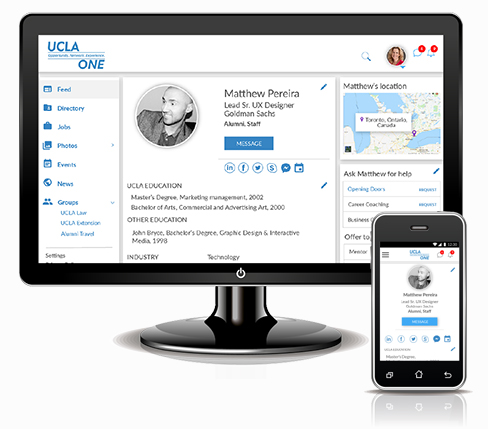
\includegraphics[width=13cm]{slike/izgledUCLAgraduwayRjesenja.png}
	\caption{Izgled UCLA Graduway rješenja}
	\label{fig:ucla-graduway}
\end{figure}

\section{VeryConnect}
VeryConnect je nešto manje popularna platforma za upravljanje svršenicima, ali sa jednako opširnim funkcionalnostima. Ima znatno manji broj klijenata od kojih je samo jedno sveučilište, University of Glasgow. Također ima neku početnu cijenu koja za razliku od Graduway-a nije javno vidljiva, a dodatne funkcionalnosti se naplaćuju zasebno.

\begin{figure}[H]
	\centering
	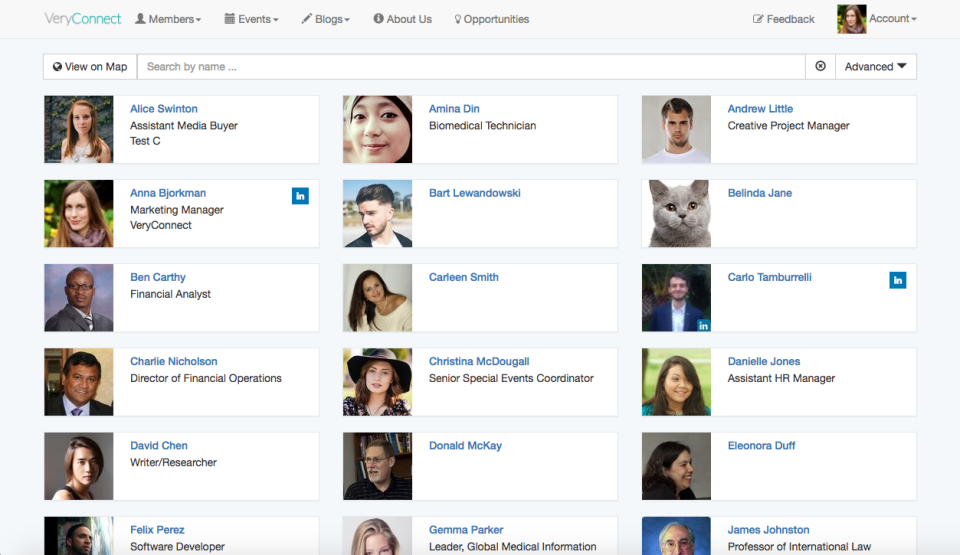
\includegraphics[width=13cm]{slike/very-connect-korisnici.png}
	\caption{VeryConnect - pregled korisnika}
	\label{fig:veryconn-users}
\end{figure}

\begin{figure}[H]
	\centering
	
\includegraphics[width=13cm]{slike/very-connect-dogadaji.png}
	\caption{VeryConnect - pregled događaja}
	\label{fig:veryconn-events}
\end{figure}

\section{Hiverbrite}
Hiverbrite je također platforma sa vrlo opširnim funkcionalnostima.

\begin{figure}[H]
	\centering
	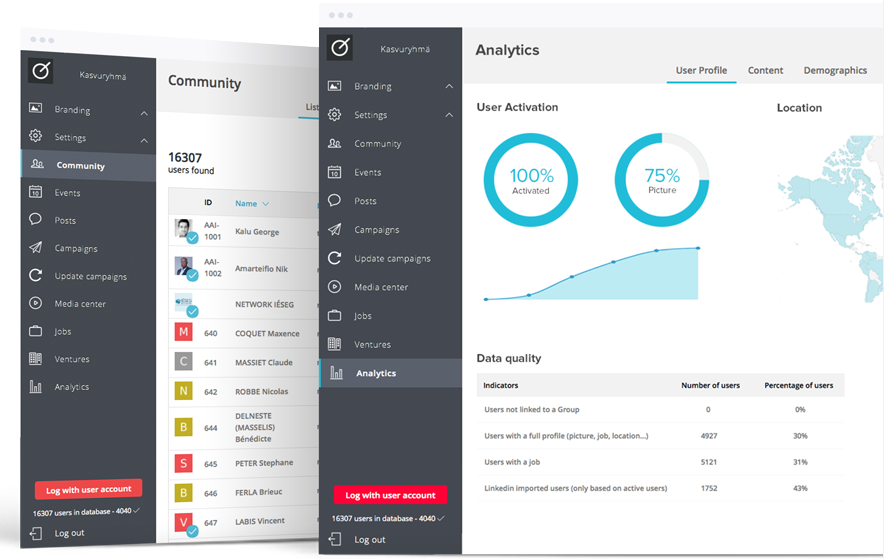
\includegraphics[width=13cm]{slike/hiverbrite-upravljanje.png}
	\caption{Izgled Hiverbrite stranice za upravljanje zajednicom}
	\label{fig:hiverbrite-menagements}
\end{figure}

\chapter{Zahtjevi nad programskom potporom}
Zahtjevi nad programskom potporom dijele se na funkcionalne zahtjeve – ono što korisnik očekuje od sustava i osnovne potrebe zbog kojih korisnik želi programsku potporu, te nefunkcionalne zahtjeve – ograničenja sustava i način na koji sustav treba biti izveden.

\section{Funkcionalni zahtjevi}
Funkcionalni zahtjevi su izjavljeni u prirodnom jeziku u obliku slučajeva korištenja, forma svakog slučaja korištenja: naziv slučaja korištenja – glavni sudionik.

 
\begin{itemize}
	\item Pregled postova - korisnik
	\item Dodavanje posta - administrator
	\item Brisanje posta - administrator
	\item Uređivanje posta - administrator
	\item Filtriranje postova po tipu - korisnik
	\item Pregled korisničkog računa - korisnik
	\item Dodavanje korisničkog računa (registracija) - anonimni korisnik
	\item Brisanje korisničkog računa - korisnik 
	\item Uređivanje korisničkog računa - korisnik
 	\item Pregled svih korisnika - administrator
	\item Prijava na sustav - korisnik 
	\item Odjava sa sustava - korisnik
\end{itemize}

\section{Nefunkcionalni zahtjevi}
Nefunkcionalni zahtjevi su sljedeći:

\begin{itemize}
	\item Sustav mora podržavati istodobni rad više korisnika
	\item Sustav mora biti otporan na kritične pogreške
	\item Sustav mora biti otporan na XSS ranjivosti
	\item Sustav mora biti ostvaren MVC arhitekturom kao web aplikacija
	\item Sustav mora biti u mogućnosti spremati podatke u bazu podataka
\end{itemize}

\chapter{Arhitektura sustava}
\section{Baza podataka}
\subsection{Konceptualni model baze podataka}

\subsection{Fizički model baze podataka}


\chapter{Zaključak}
Zaključak.

\bibliography{literatura}
\bibliographystyle{fer}

\begin{sazetak}
	Sažetak na hrvatskom jeziku.
		
	\kljucnerijeci{Ključne riječi, odvojene zarezima.}
\end{sazetak}

% TODO: Navedite naslov na engleskom jeziku.
\engtitle{Title}
\begin{abstract}
	Abstract.
		
	\keywords{Keywords.}
\end{abstract}

\end{document}
